\section[检查观测值]{检查观测值\\Investigations of the Observations}
在处理复杂的RTK码观测值之前,我们把数据处理过程分为更小的Ⅰ、Ⅱ、Ⅲ步。如何同时利用码观测值和载波观测值估计基线向量是个大问题,下面将使用不同的工具演示解决这个问题的更多方法。

\subsection{10.5.1电离层延迟}

\uppercase\expandafter{\romannumeral1}、对于基础方程(10.9)里的观测值$P_{1}$,$\Phi_{1}$,$P_{2}$和$\Phi_{2}$,我们使用第二个和第四个观测值并且处理的是双差观测方程
\begin{equation}
	\begin{split}
		\Phi_{1}=\rho^{*}-I+\lambda_{1}N^{1}-\epsilon_{1}\\
		\Phi_{2}=\rho^{*}-I+\lambda_{2}N^{2}-\epsilon_{2}
	\end{split}
\end{equation}
忽略误差项 $\epsilon_{i}$ ,消掉$\rho^{*}$可得到电离层延迟的表达式

\begin{equation}
	I=\frac{(\Phi_{2}-\lambda_{2}N_{2})-(\Phi_{1}-\lambda_{1}N_{1})}{1-\alpha}
\end{equation}

\begin{figure}
	\centering
	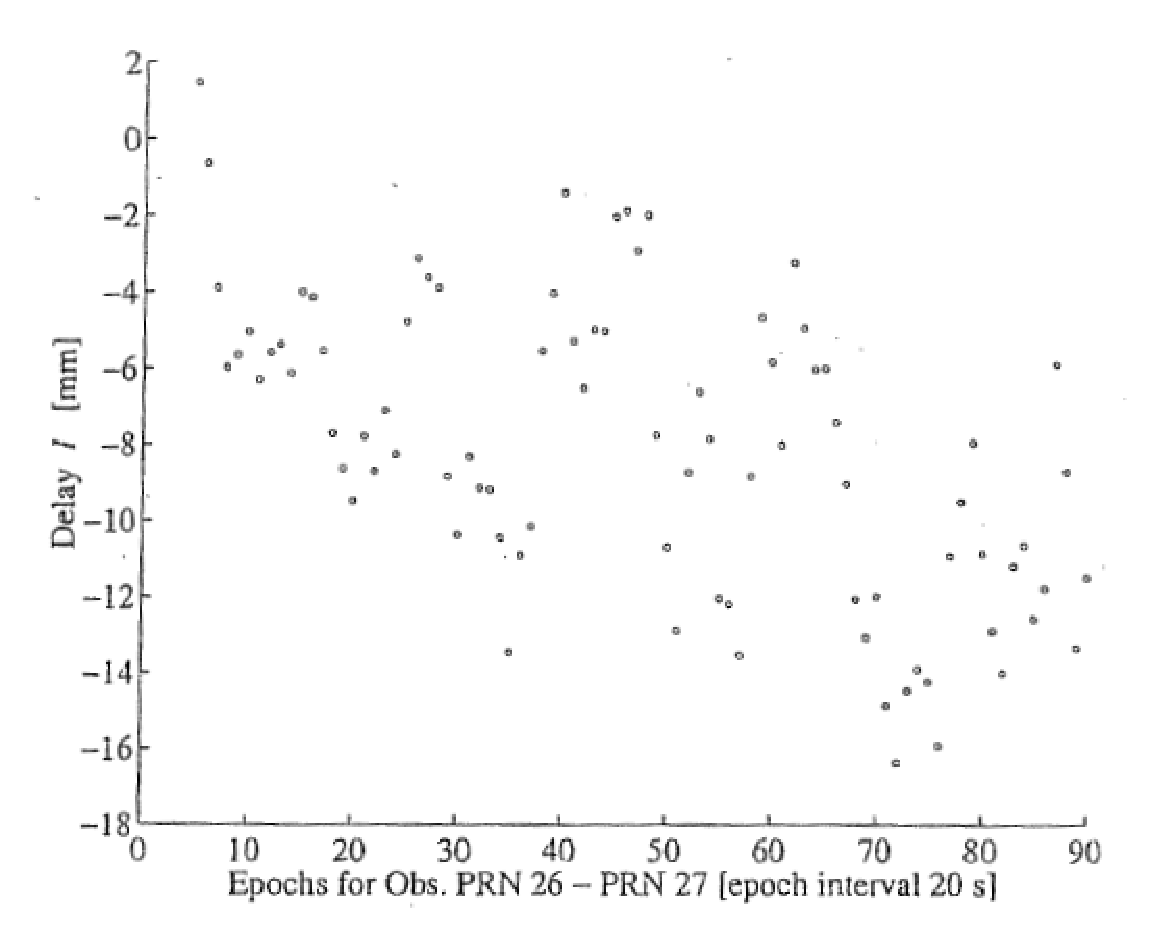
\includegraphics[width=0.4\linewidth]{TeX_files/Part03/chapter10/image/9-7}
	\caption{按照公式(10.21)对于相位双差,电离层延迟变化为2mm到-16mm,基线长度为4.6km}
	\label{fig:9-7}
\end{figure}

电离层延迟变化如图10.7,变化值很分散,在几个厘米以内。因此通过实验可以确定在I=0(没有延迟)的情况下是否能够被接受。

利用(10.20)的两个方程可以消掉电离层延迟项I,得到
\begin{equation}
	60\Phi_{1}/\lambda_{1}-77\Phi_{2}/\lambda_{2}=60N_{1}-77N_{2}
\end{equation}

因为$\frac{f_{1}}{f_{2}}=\frac{154}{120}=\frac{77}{60}$,所以出现系数60和70。但同时如此大的系数扩大了噪声。

\uppercase\expandafter{\romannumeral2}、另外一种消除电离层延迟I的方法是使用双频观测值。电离层延迟从几米到十几米变化不等。幸运的是电离层延迟是分散的,它取决于频率f。利用方程(10.8)我们可以获得双频电离层改正。首先利用同一颗卫星搭载在L1和L2载波上的两个伪距观测值:
$$
P_{1}=\rho^{*}+I-e_{1}
$$
$$
P_{2}=\rho^{*}+\alpha I-e_{2}
$$\\
忽略误差项 $e_{i}$,消掉I可得到理想伪距$\rho^{*}$:
$$
\rho^{*}=P_{1}-\frac{P_{1}-P_{2}}{1-\alpha}=P_{1}+1.545727802(P_{1}-P_{2})
$$\\
这个伪距的线性组合被称为消电离层组合。

\uppercase\expandafter{\romannumeral3}、接下来描述曾在第8章中使用过的一种简单的滤波方法$k_dd4$。它有4个未知量:理想伪距$\rho^{*}$,电离层延迟I和整周模糊度$N_{1}$、$N_{2}$。我们观测双频码伪距P和码相位$\Phi$。重写(10.9)如下:
$$
\begin{bmatrix}
1&1&0&0\\
1&-1&\lambda_{1}&0\\
1&\alpha&0&0\\
1&-\alpha&0&\lambda_{2}
\end{bmatrix}
\begin{bmatrix}
\rho^{*}\\I\\N_{1}\\N_{2}
\end{bmatrix}
=
\begin{bmatrix}
P_{1}\\\Phi_{1}\\P_{2}\\\Phi_{2}
\end{bmatrix}
-e
$$\\
独立观测值$P_{1}$,$\Phi_{1}$,$P_{2}$和$\Phi_{2}$的方差为$0.3^{2}$,$0.005^{2}$,$0.3^{2}$和$0.005^{2}m^{2}$。给出的$x_{0}$初始值,利用5个历元解含有4个未知量的4个方程。由于接收机的冷启动,早期的数据含有相当大的噪声。对于误差$\epsilon$的状态方程中$\rho^{*}$ ,I和模糊度的方差为100, 10, 0和0$m^{2}$,则输出结果包含 $\rho^{*}$,I,$N_{1}$和宽巷模糊度$N_{w}=N_{1}-N^{2}$的滤波值。

电离层延迟的绝对值变化非常剧烈,它取决于季节、纬度、这一天的时间以及其他参数。关于电离层的更多研究在Klobuchar 模型中(1996)进行了阐述。

\subsection{10.5.2 电离层延迟}

在纬度为$\varphi$的地区接收到的GPS信号的电离层延迟模型如下,其中天顶距离为 z = $90^{\circ}$-h。大气压力$P_{0}$ 的单位为豪巴,高度H的单位为千米,温度$T_{0}$的单位为开尔文,水汽分压$e_{0}$的单位为豪巴,则
\begin{equation}
	T=0.002277\frac{1+0.0026cos2\varphi+0.00028H}{cosz}(P_{0}+(\frac{1255}{T_{0}}+0.05)e_{0}).
\end{equation}\\

这个简单的模型可以以不同的方式被扩展。我们的目的是确定短基线向量并达到厘米级精度,而M-file 对流层计算程序能轻易满足这个要求,计算的天顶对流层延迟T$\approx$2.4 m。从公式可以看出对流层延迟与cosz成反比,因此在处理GPS观测数据时,截止高度角通常选为$15^{\circ}$。

M-file 对流层计算程序需要以下参数作为输入:

- sinel  卫星仰角的正弦,

- hsta  以千米为单位的测站高,高度hp以豪巴为单位的大气压力p,

- tkel  高度为htkel以开尔文为单位的表面温度,

- hum  高度为hhum以百分比为单位的湿度,

- hp  以千米为单位的进行压力测量的高度,

- htkel  以千米为单位的进行温度测量的高度和

- hhum  以千米为单位的进行湿度测量的高度。

这个对流层计算代码可能是最近出版的代码中对流层延迟计算结果最精密的。

天顶对流层延迟具有2\%的不确定性甚至更小。当天顶距小于$75^{\circ}$时,这个不确定性并不会增加很多。如果所有的伪距观测值含有的是一个常数偏差,那么计算的位置将不会受到影响,而仅仅是扩大了接收机钟差的偏差。但是如果对流层延迟不是常数,这将会影响定位点的高度。然而,对于短基线双差定位对流层延迟并不是很大的误差。

\subsection{10.5.3 码观测值上的多路径}

多路径效应是指卫星信号沿着多个路径到达接收机天线的情况。卫星发射的信号大部分直接达到接收机,但是部分信号受到周围表面的反射后才到达接收机。多路径效应取决于卫星的几何分布和接收机天线所处的环境,因此很难通过模型确定。24小时的长时间观测在一定程度上可以减小多路径效应的影响,而对于短时间观测,多路径效应是一个不可忽视的问题。

更多关于如何计算多路径效应的细节可参见\textbf{291(根据排版找到相应页码)}页。